\documentclass[tikz,border=10mm]{standalone}
\usetikzlibrary{calc}

\def\xw{2}
\def\yw{7}
\def\rad{5.0mm}
\def\dist{20.0mm}
\def\edge{10.0mm}

\begin{document}
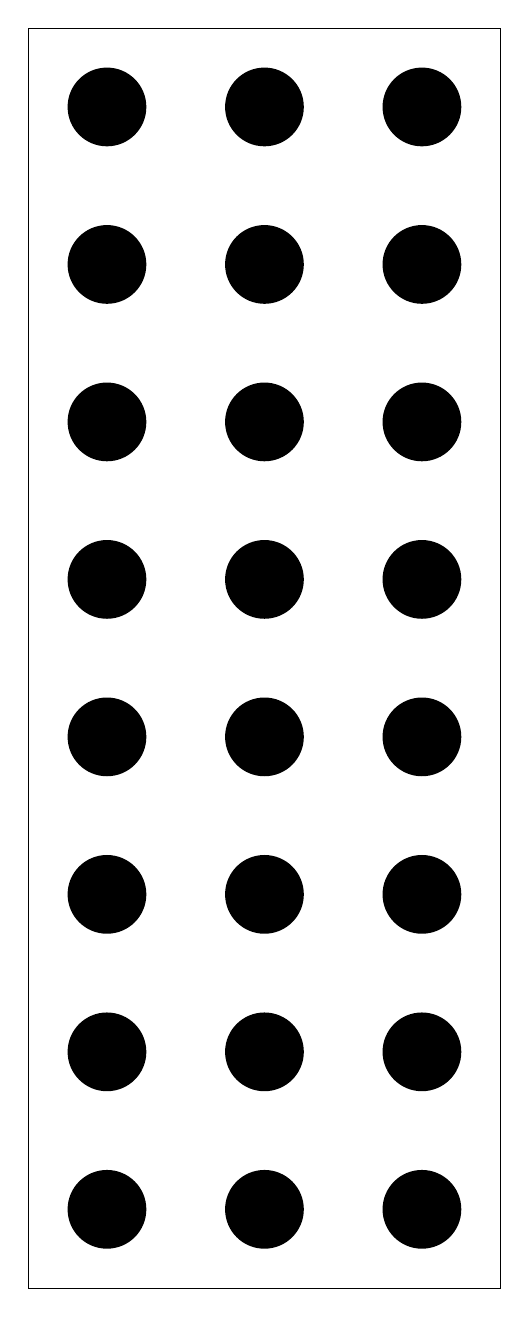
\begin{tikzpicture}[scale=1]



%This circle grid pattern is 2.4"x7" (60.9 mm x 177.8 mm).
%The circle radius is \rad,


\draw ( 0mm ,0mm) rectangle (\xw*\dist+\edge+\edge,\yw*\dist +\edge+\edge);

\foreach \b in {0,...,\xw}{
   \foreach \c in {0,...,\yw}{
      \fill[black] (\b*\dist+\edge,\c*\dist+\edge) circle [radius=\rad] ;

    }

}


\end{tikzpicture}
\end{document}
